\documentclass[14pt,a4paper]{extarticle}

% Поддержка различных компиляторов (pdfLaTeX, XeLaTeX, LuaLaTeX) на Overleaf
\usepackage{iftex}
\ifPDFTeX
  \usepackage[T2A]{fontenc}
  \usepackage[utf8]{inputenc}
  \usepackage[russian]{babel}
  \usepackage{tempora}
  \usepackage{courier}
\else
  \usepackage{fontspec}
  \defaultfontfeatures{Ligatures=TeX}
  \setmainfont{Times New Roman}
  \setmonofont{Courier New}
  \usepackage{polyglossia}
  \setmainlanguage{russian}
\fi

\usepackage{amsmath,amssymb}
\usepackage{graphicx}
\usepackage{caption}
\usepackage{booktabs}
\usepackage{listings}
\usepackage{xcolor}
\usepackage{geometry}
\usepackage{setspace}
\usepackage{indentfirst}
\usepackage{fancyhdr}
\usepackage{microtype}
\usepackage{tabularx}
\usepackage{float}

% Поля страницы по стандарту БГУИР СТП 01-2017 (Приложение Л)
\geometry{
  a4paper,
  left=30mm,
  right=15mm,
  top=20mm,
  bottom=20mm,
  footskip=12mm
}

% Межстрочный интервал 1.5, абзацный отступ 1.25 см
\setstretch{1.5}
\setlength{\parindent}{12.5mm}
\setlength{\parskip}{0pt}

% Нумерация страниц: в правом нижнем углу со 2-й страницы арабскими цифрами
\pagestyle{fancy}
\fancyhf{}
\fancyfoot[R]{\thepage}
\renewcommand{\headrulewidth}{0pt}
\renewcommand{\footrulewidth}{0pt}

% Форматирование подписей к рисункам и таблицам по СТП 01-2017
\DeclareCaptionLabelSeparator{emdash}{\ --- }
\captionsetup[figure]{
  name=Рисунок,
  labelsep=emdash,
  justification=centering,
  font={normalsize},
  skip=6pt
}
\captionsetup[table]{
  name=Таблица,
  labelsep=emdash,
  justification=raggedleft,
  singlelinecheck=false,
  font={normalsize},
  skip=6pt
}

% Настройка оформления кода программ: Courier New 9 пт, без рамок
\lstset{
  basicstyle=\fontsize{9pt}{10pt}\ttfamily,
  breaklines=true,
  breakatwhitespace=true,
  keepspaces=true,
  numbers=none,
  frame=none,
  showstringspaces=false,
  tabsize=4,
  keywordstyle=\bfseries\color{black},
  commentstyle=\color{black},
  stringstyle=\color{black}
}

\begin{document}

% ==============================================================================
% ТИТУЛЬНЫЙ ЛИСТ (БГУИР СТП 01-2017)
% ==============================================================================
\begin{titlepage}
\thispagestyle{empty}
\begin{center}
  \setstretch{1.1}
  МИНИСТЕРСТВО ОБРАЗОВАНИЯ РЕСПУБЛИКИ БЕЛАРУСЬ \\
  БЕЛОРУССКИЙ ГОСУДАРСТВЕННЫЙ УНИВЕРСИТЕТ ИНФОРМАТИКИ И РАДИОЭЛЕКТРОНИКИ \\
  Факультет компьютерных систем и сетей \\
  Кафедра программного обеспечения информационных технологий \\
  \vspace{60mm}

  {\large \textbf{ОТЧЕТ}}\\
  \vspace{3mm}
  {\large \textbf{ПО ЛАБОРАТОРНОЙ РАБОТЕ № 4}}\\
  \vspace{3mm}
  {\normalsize \textbf{«КЛАССИФИКАЦИЯ ДАННЫХ. ЛОГИСТИЧЕСКАЯ РЕГРЕССИЯ, МЕТОД ОПОРНЫХ ВЕКТОРОВ И РЕШАЮЩИЕ ДЕРЕВЬЯ»}}\\
  \vspace{4mm}
  {\normalsize Дисциплина: «Методы машинного обучения»}\\
  \vspace{2mm}
  {\normalsize Вариант № 7}
\end{center}

\vspace{45mm}

\begin{flushright}
  \setstretch{1.2}
  \begin{tabular}{ll}
    \textbf{Выполнил:} & студент гр. 351002 \\
    & \textbf{Власовец А. И.} \\
    \textbf{Проверил:} & ассистент кафедры ПОИТ \\
    & \textbf{Лебедевич А. В.}
  \end{tabular}
\end{flushright}

\vfill

\begin{center}
  Минск 2026
\end{center}
\end{titlepage}

\setcounter{page}{2}

% ==============================================================================
% ЦЕЛЬ РАБОТЫ И ИНДИВИДУАЛЬНОЕ ЗАДАНИЕ
% ==============================================================================
\section*{ЦЕЛЬ РАБОТЫ}
\addcontentsline{toc}{section}{ЦЕЛЬ РАБОТЫ}

Приобретение практических навыков решения прикладных задач бинарной классификации данных с использованием ключевых алгоритмов контролируемого машинного обучения: логистической регрессии, метода опорных векторов (Support Vector Machines, SVM с линейным и радиальным RBF-ядром) и решающих деревьев CART. Исследование методов предобработки финансовых признаков, оценки обобщающей способности моделей по комплексной системе метрик (Accuracy, Precision, Recall, $F_1$-score, ROC-AUC, PR-AUC), визуализации разделяющих гиперповерхностей и практического скоринга потенциальных заемщиков.

\section*{ИНДИВИДУАЛЬНОЕ ЗАДАНИЕ (ВАРИАНТ № 7)}
\addcontentsline{toc}{section}{ИНДИВИДУАЛЬНОЕ ЗАДАНИЕ}

В соответствии с учебной программой дисциплины «Методы машинного обучения» и вариантом № 7 необходимо выполнить:
\begin{enumerate}
  \item Выполнить разведочный анализ и первичную очистку данных банковского кредитного скоринга (\texttt{Bankloan.csv}), исследовать соотношение классов, пропуски и распределения признаков.
  \item Произвести разделение выборки на обучающую ($80\%$) и контрольную ($20\%$) части со стратификацией по целевому классу (\texttt{default}), выполнить стандартизацию количественных признаков (\texttt{StandardScaler}).
  \item Обучить модель логистической регрессии, проанализировать весовые коэффициенты, отношение шансов (Odds Ratios) и характер разделяющей границы.
  \item Построить классификаторы методом опорных векторов с линейным ядром (\texttt{LinearSVC} / \texttt{SVC(kernel='linear')}) и нелинейным гауссовым ядром (\texttt{SVC(kernel='rbf')}), определить опорные векторы и геометрический зазор разделения.
  \item Построить решающее дерево алгоритма CART (\texttt{DecisionTreeClassifier}) с регулировкой глубины для предотвращения переобучения, визуализировать структуру ветвления и рассчитать информативность признаков по критерию Джини.
  \item Построить матрицы ошибок (Confusion Matrices), кривые ошибок ROC и точности-полноты PR для всех моделей, сопоставить их качество.
  \item Применить наилучшую построенную модель для скоринга 450 новых кандидатов кредитного портфеля и выдать рекомендации о выдаче либо отказе в предоставлении займа.
\end{enumerate}

% ==============================================================================
% ТЕОРЕТИЧЕСКИЕ СВЕДЕНИЯ
% ==============================================================================
\section*{ТЕОРЕТИЧЕСКИЕ СВЕДЕНИЯ}
\addcontentsline{toc}{section}{ТЕОРЕТИЧЕСКИЕ СВЕДЕНИЯ}

\subsection*{1. Задача бинарной классификации и логистическая регрессия}

В задаче бинарной классификации объекту $x \in \mathbb{R}^d$ ставится в соответствие метка класса $y \in \{0, 1\}$. Модель логистической регрессии оценивает апостериорную вероятность принадлежности объекта к положительному классу $P(y=1|x)$ посредством сигмоидной функции активации:
\begin{equation}
  P(y = 1 | x) = \sigma(w^T x + b) = \frac{1}{1 + e^{-(w^T x + b)}},
\end{equation}
где $w \in \mathbb{R}^d$ --- вектор весов признаков, $b \in \mathbb{R}$ --- свободный член (смещение).

Отношение шансов (Odds Ratio) для $j$-го признака показывает, во сколько раз изменяются шансы наступления события $y=1$ при увеличении признака $x_j$ на единицу:
\begin{equation}
  \text{OR}_j = \exp(w_j).
\end{equation}
Обучение проводится методом максимального правдоподобия через минимизацию функции логистических потерь (Binary Cross-Entropy / Log-Loss) с $L_2$-регуляризацией:
\begin{equation}
  \mathcal{L}(w, b) = -\frac{1}{l} \sum_{i=1}^l \left[ y_i \ln \sigma(w^T x_i + b) + (1 - y_i) \ln(1 - \sigma(w^T x_i + b)) \right] + \frac{1}{2C} \|w\|_2^2.
\end{equation}

\subsection*{2. Метод опорных векторов (SVM)}

Метод опорных векторов строит оптимальную гиперплоскость $w^T x + b = 0$, максимизирующую геометрический зазор $M = \frac{2}{\|w\|_2}$ между разделяемыми классами при штрафе за нарушение границы:
\begin{equation}
  \min_{w, b, \xi} \frac{1}{2} \|w\|_2^2 + C \sum_{i=1}^l \xi_i \quad \text{при условиях} \quad y_i(w^T x_i + b) \ge 1 - \xi_i, \quad \xi_i \ge 0.
\end{equation}
Для нелинейно разделимых данных применяется метод ядер (Kernel Trick). Наиболее универсальным является радиально-базисное ядро (RBF):
\begin{equation}
  K(x_i, x_j) = \exp(-\gamma \|x_i - x_j\|^2), \quad \gamma = \frac{1}{2\sigma^2}.
\end{equation}

\subsection*{3. Решающие деревья (CART)}

Алгоритм CART (Classification and Regression Trees) строит бинарное решающее дерево путем рекурсивного разбиения пространства признаков. В каждом узле выбирается признак $j$ и порог разбиения $t$, максимизирующие снижение неоднородности Джини:
\begin{equation}
  G(S) = 1 - \sum_{k=1}^K p_k^2, \quad \Delta G(S, j, t) = G(S) - \frac{|S_L|}{|S|} G(S_L) - \frac{|S_R|}{|S|} G(S_R),
\end{equation}
где $p_k$ --- доля объектов класса $k$ в вершине $S$.

\subsection*{4. Метрики качества классификации}

Для несбалансированных выборок ключевыми показателями выступают элементы матрицы ошибок: $TP$ (истинно-положительные), $FP$ (ложно-положительные), $FN$ (ложно-отрицательные), $TN$ (истинно-отрицательные). На их основе рассчитываются:
\begin{equation}
  \text{Accuracy} = \frac{TP + TN}{TP + TN + FP + FN}, \quad \text{Precision} = \frac{TP}{TP + FP},
\end{equation}
\begin{equation}
  \text{Recall} = \frac{TP}{TP + FN}, \quad F_1 = 2 \cdot \frac{\text{Precision} \cdot \text{Recall}}{\text{Precision} + \text{Recall}}.
\end{equation}
Площадь под ROC-кривой (ROC-AUC) характеризует вероятность того, что случайно выбранному положительному объекту классификатор присвоит более высокий скор вероятности, чем случайно выбранному отрицательному.

% ==============================================================================
% ПРАКТИЧЕСКАЯ РЕАЛИЗАЦИЯ И РЕЗУЛЬТАТЫ
% ==============================================================================
\section*{ПРАКТИЧЕСКАЯ РЕАЛИЗАЦИЯ И РЕЗУЛЬТАТЫ}
\addcontentsline{toc}{section}{ПРАКТИЧЕСКАЯ РЕАЛИЗАЦИЯ И РЕЗУЛЬТАТЫ}

\subsection*{1. Разведочный анализ данных (EDA)}

В качестве исследуемого набора данных использован \texttt{Bankloan.csv}, содержащий 1150 наблюдений и 9 признаков. Первые 700 строк представляют размеченную историческую выборку клиентов банка с известным фактом дефолта (\texttt{default} $\in \{0, 1\}$), а последующие 450 строк --- новые кредитные заявки, подлежащие предиктивному скорингу.

На рисунке 1 приведен структурный анализ датасета и распределение целевой переменной. В обучающей совокупности дефолт зафиксирован у 183 клиентов ($26.1\%$), тогда как добросовестными заемщиками являются 517 человек ($73.9\%$). Пропущенные значения в признаковом описании отсутствуют.

\begin{figure}[H]
  \centering
  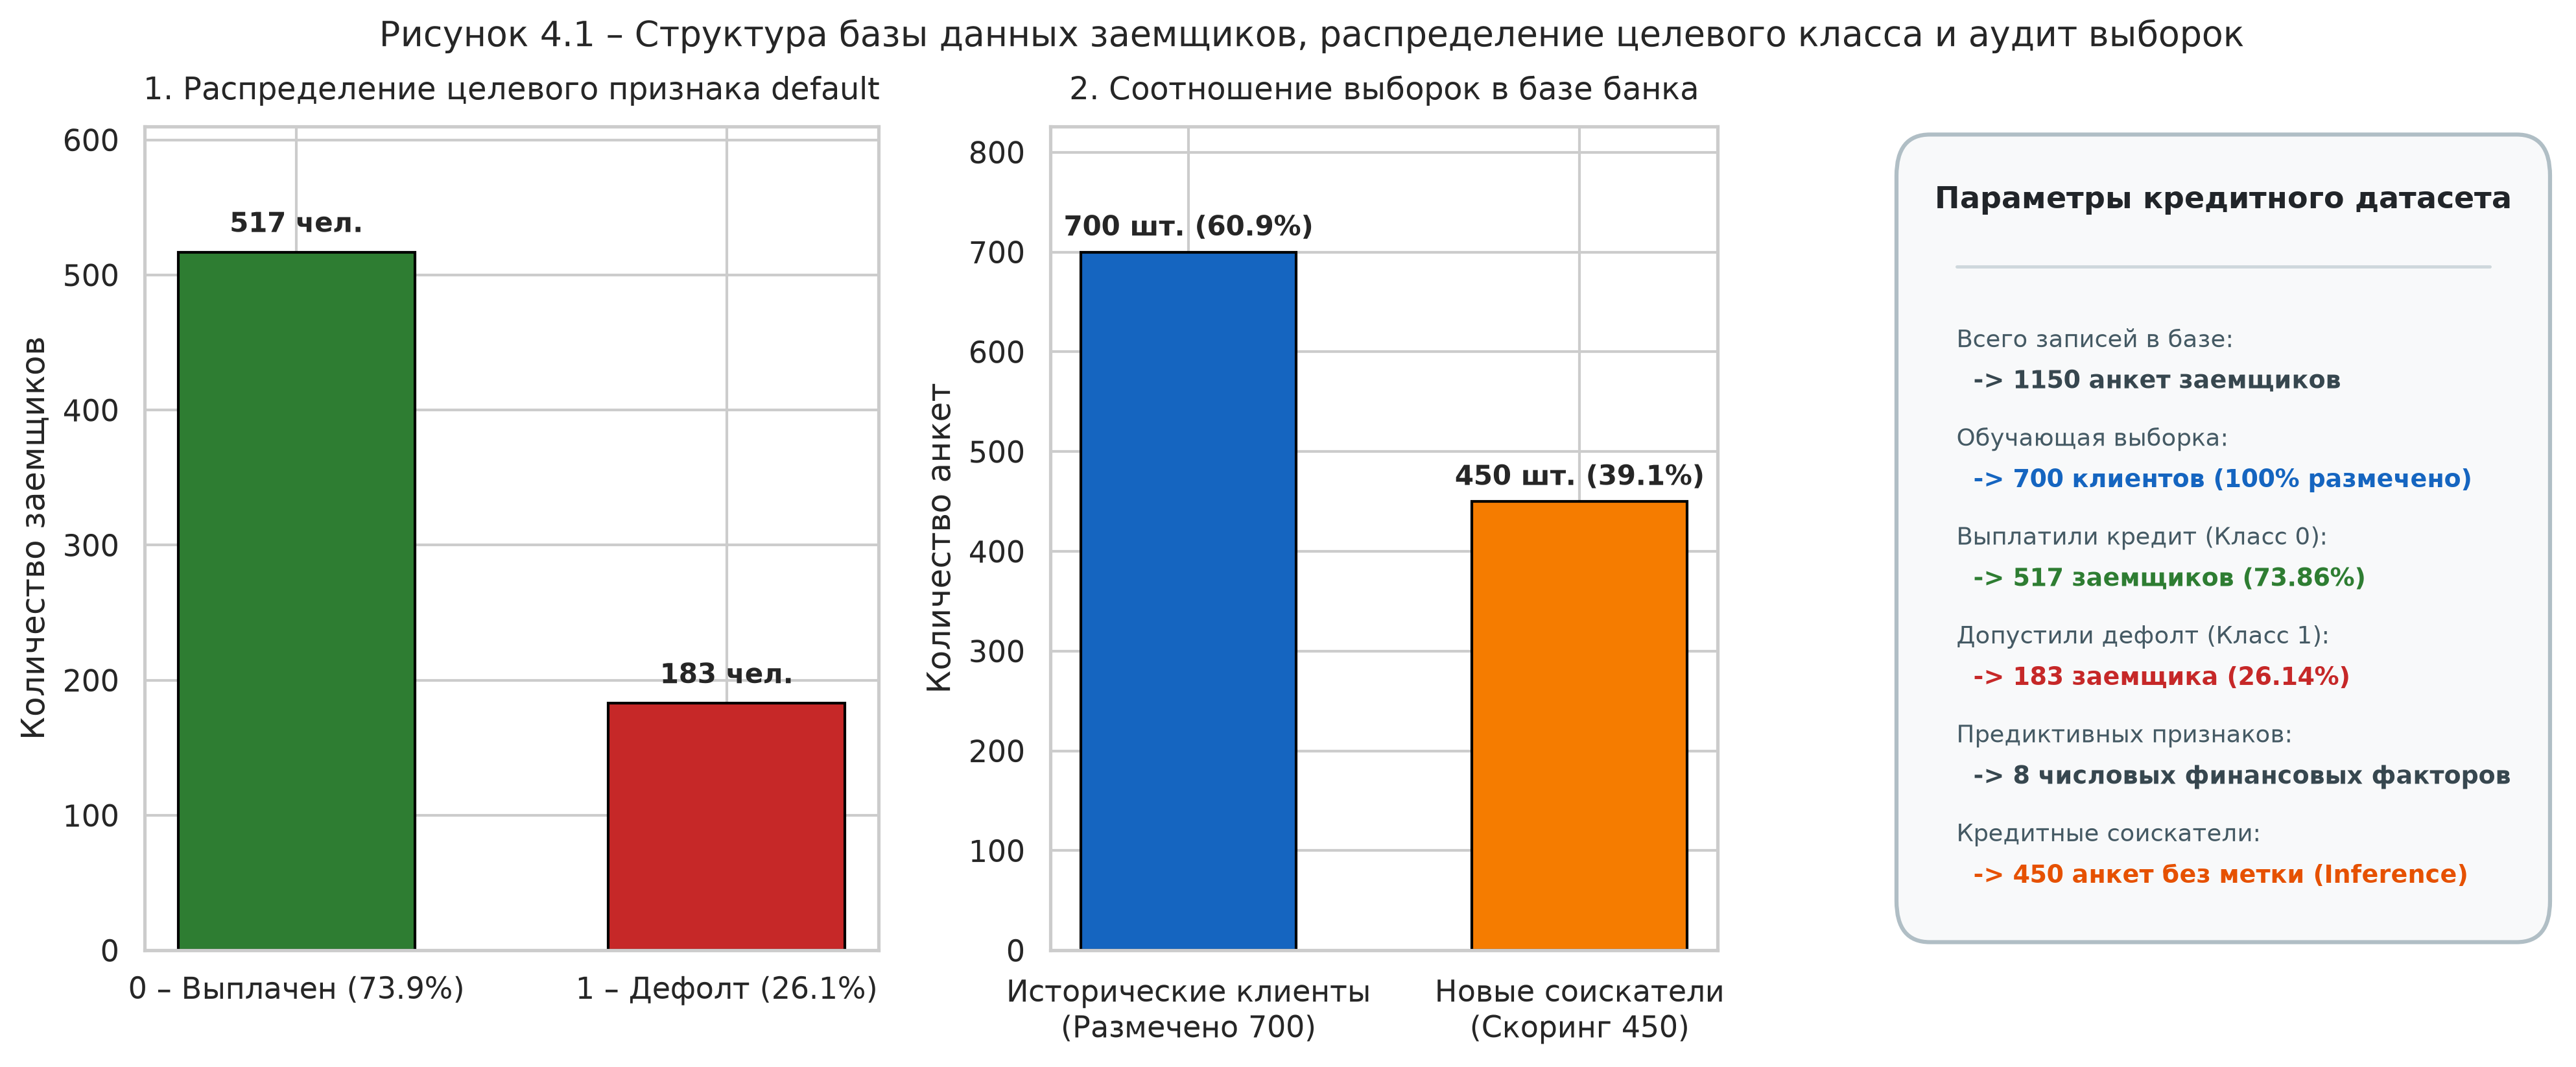
\includegraphics[width=0.92\textwidth]{plots/01_dataset_and_missing_analysis.png}
  \caption{Структура выборки, статус пропусков и баланс классов}
\end{figure}

На рисунке 2 отображены гистограммы распределений с ядерной оценкой плотности (KDE) и коробчатые диаграммы (боксплоты) для всех числовых предикторов в разрезе статуса дефолта.

\begin{figure}[H]
  \centering
  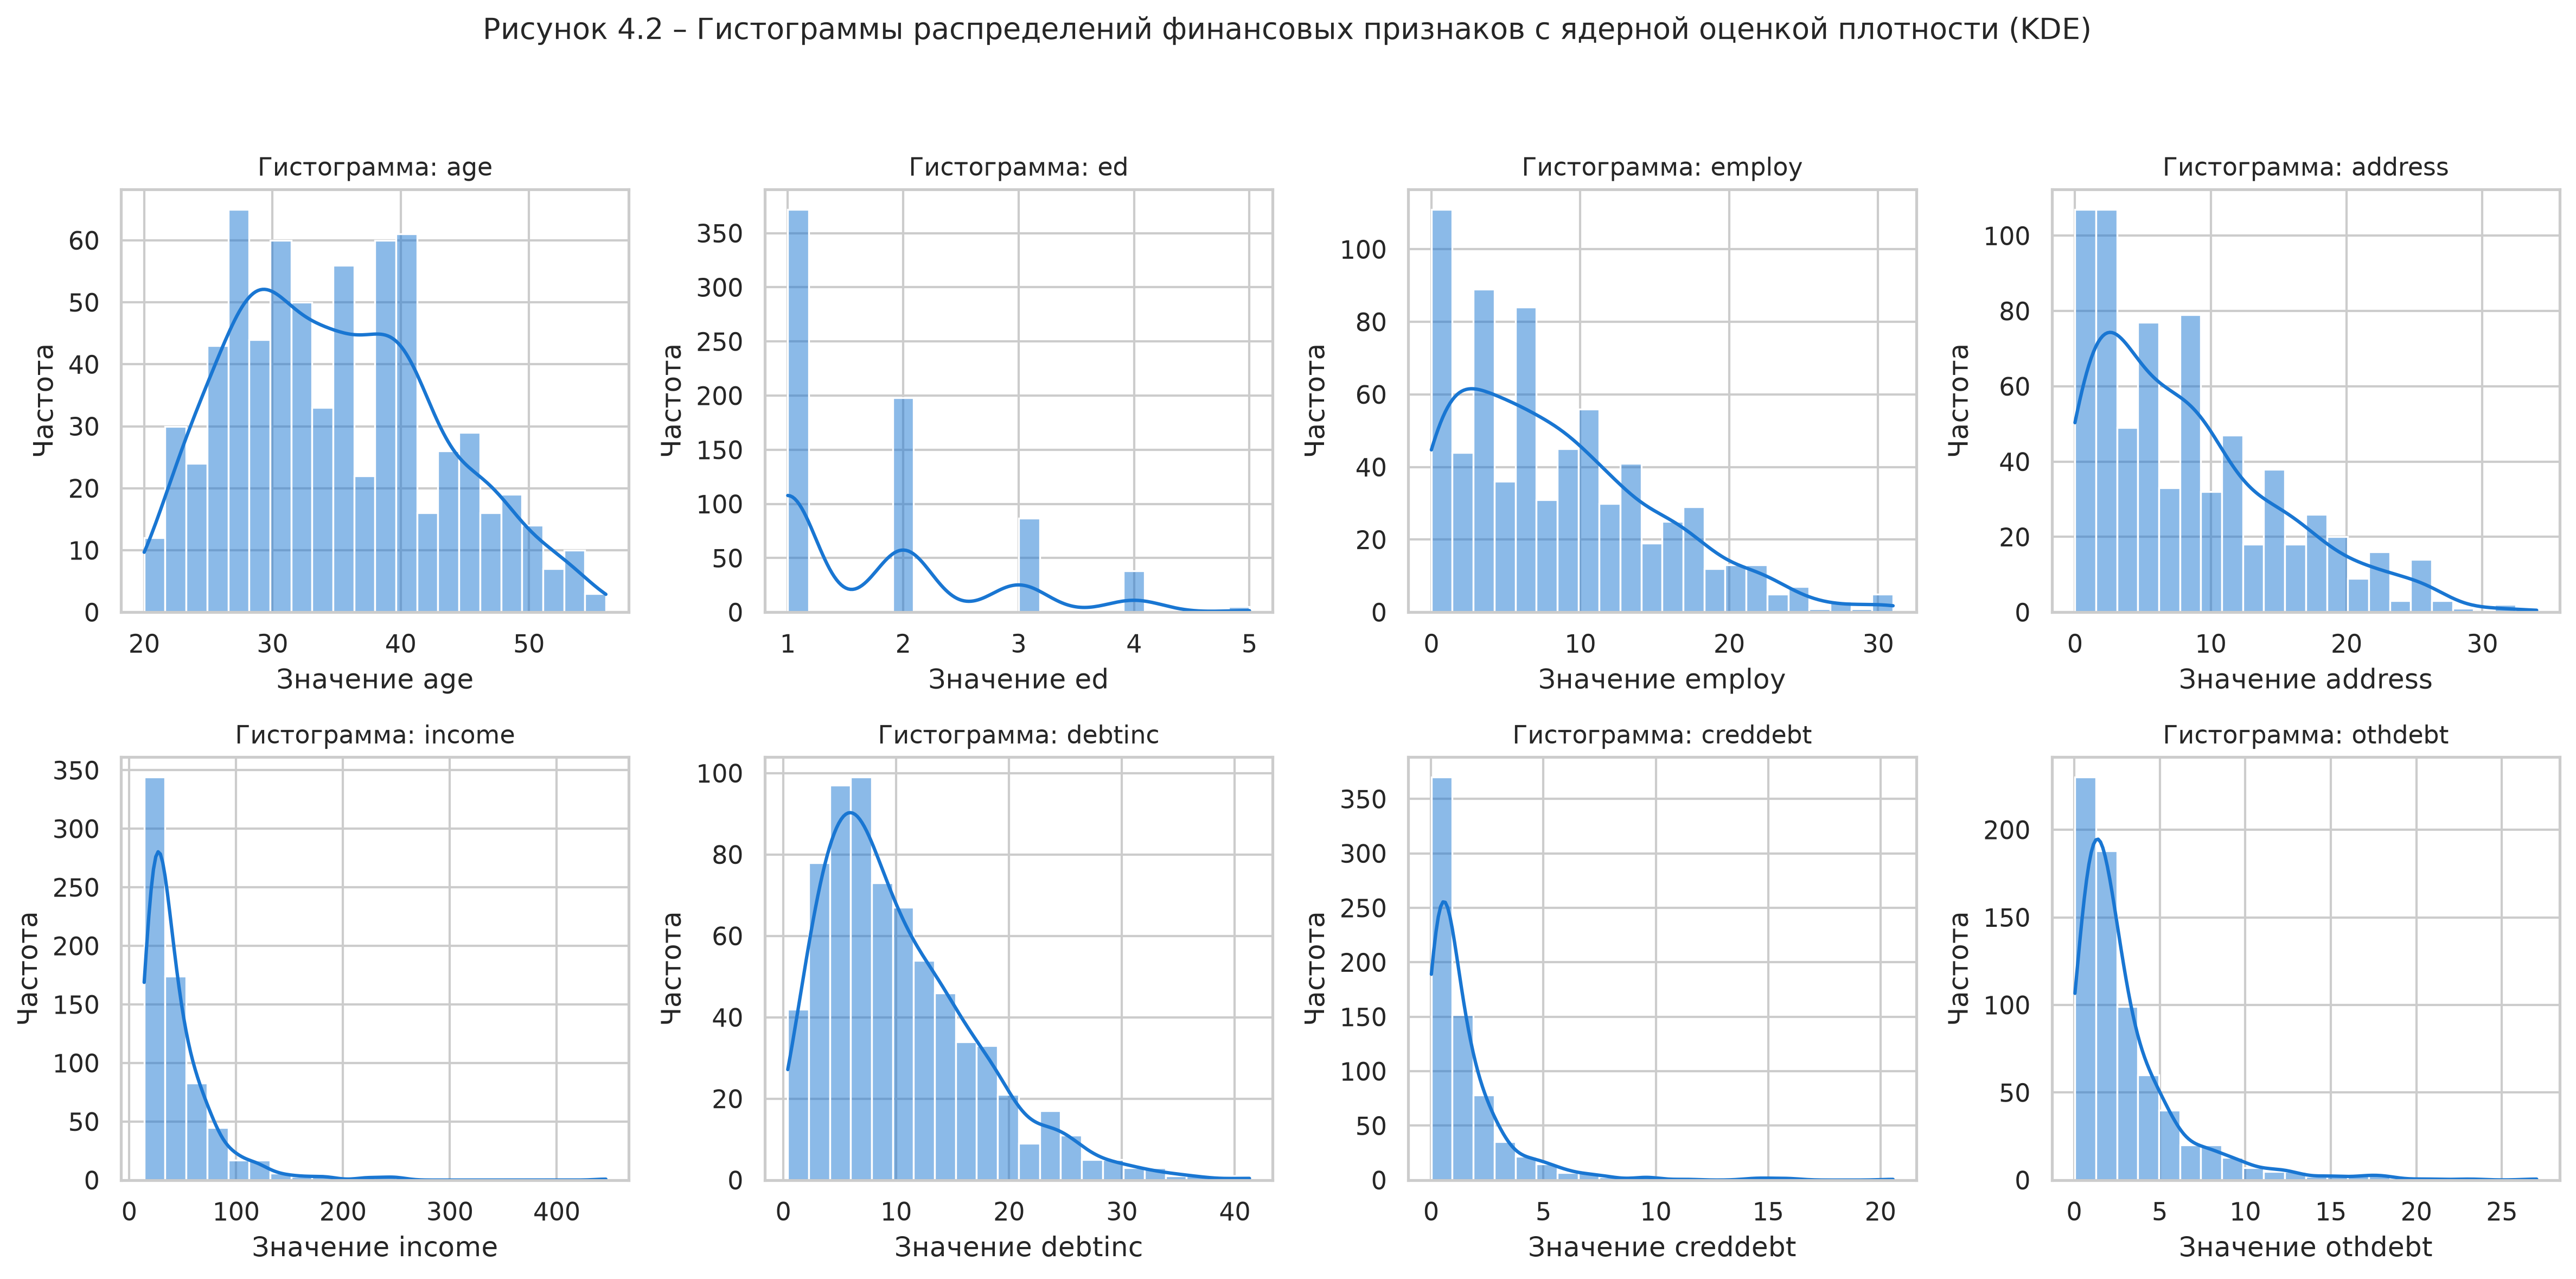
\includegraphics[width=0.92\textwidth]{plots/02_features_distributions_and_boxplots.png}
  \caption{Гистограммы и коробчатые диаграммы признаков}
\end{figure}

На рисунке 3 представлена корреляционная матрица Пирсона и диаграмма размаха межквартильного интервала. Наибольшую линейную взаимосвязь с вероятностью дефолта демонстрирует долговая нагрузка \texttt{debtinc} ($r = +0.39$), а также стаж работы \texttt{employ} ($r = -0.28$) и срок проживания по адресу \texttt{address} ($r = -0.26$).

\begin{figure}[H]
  \centering
  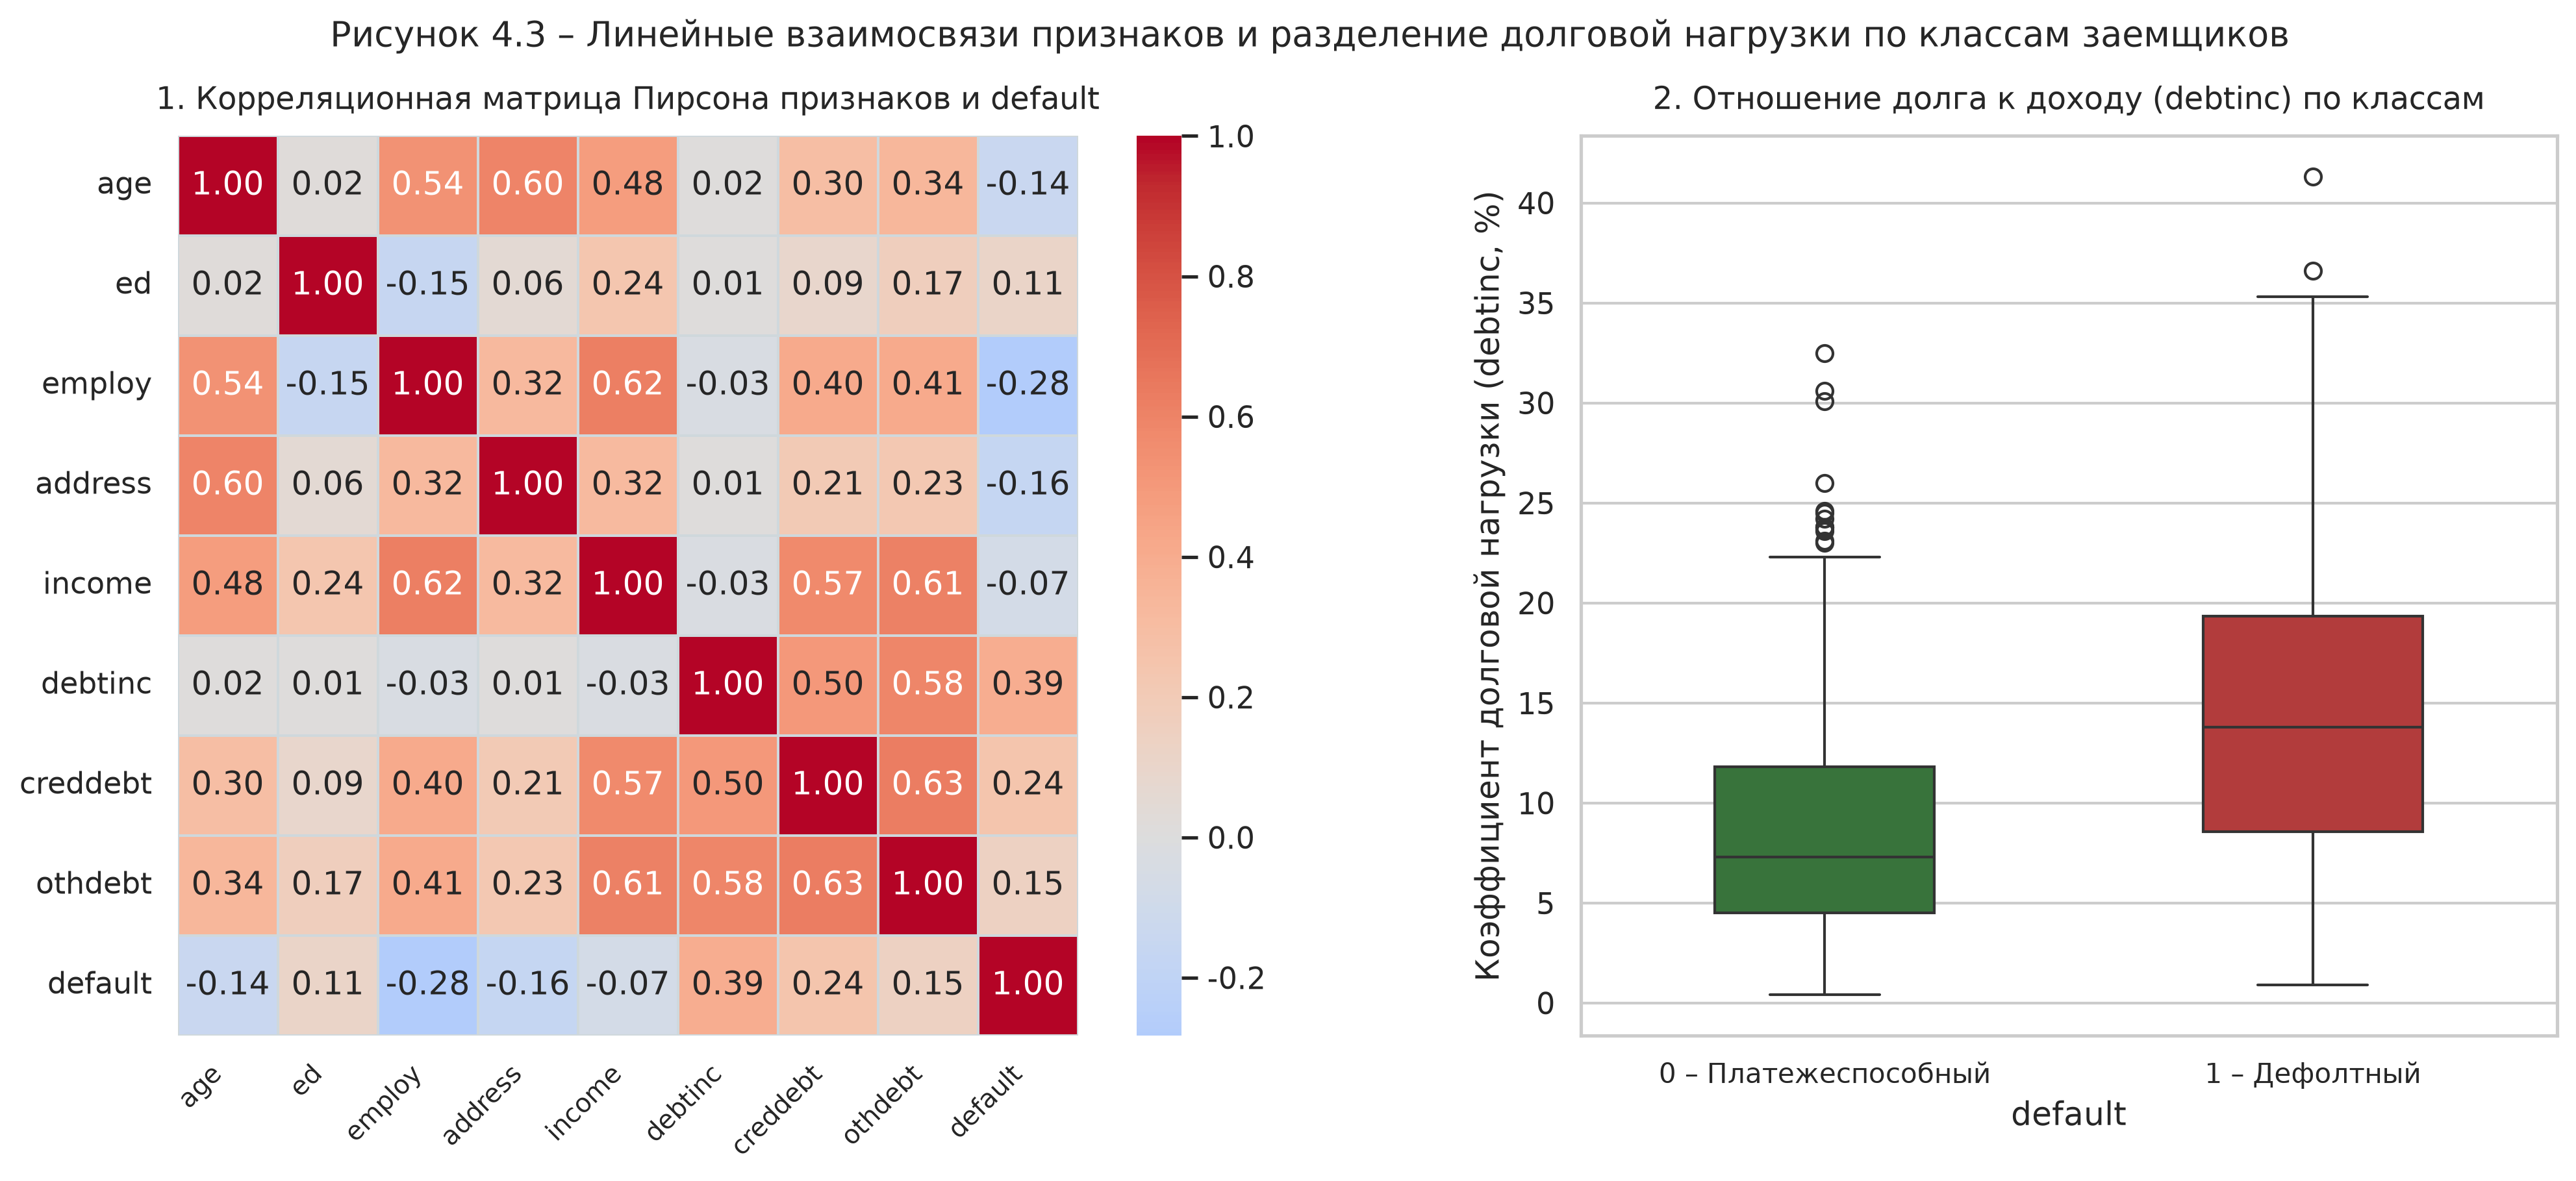
\includegraphics[width=0.92\textwidth]{plots/03_outliers_and_correlation_heatmap.png}
  \caption{Межквартильные границы выбросов и корреляционная матрица Пирсона}
\end{figure}

\subsection*{2. Логистическая регрессия}

Обучение логистической регрессии производилось на стандартизированных данных ($z = (x - \mu)/\sigma$). Полученные коэффициенты модели и отношения шансов отражены на рисунке 4. Коэффициент долговой нагрузки составляет $+0.893$ ($\text{OR} = 2.44$), что означает рост шансов невозврата в 2.44 раза при увеличении \texttt{debtinc} на одно стандартное отклонение. Напротив, каждый шаг роста стажа работы снижает шансы дефолта более чем в 2 раза ($w = -0.742, \text{OR} = 0.48$).

\begin{figure}[H]
  \centering
  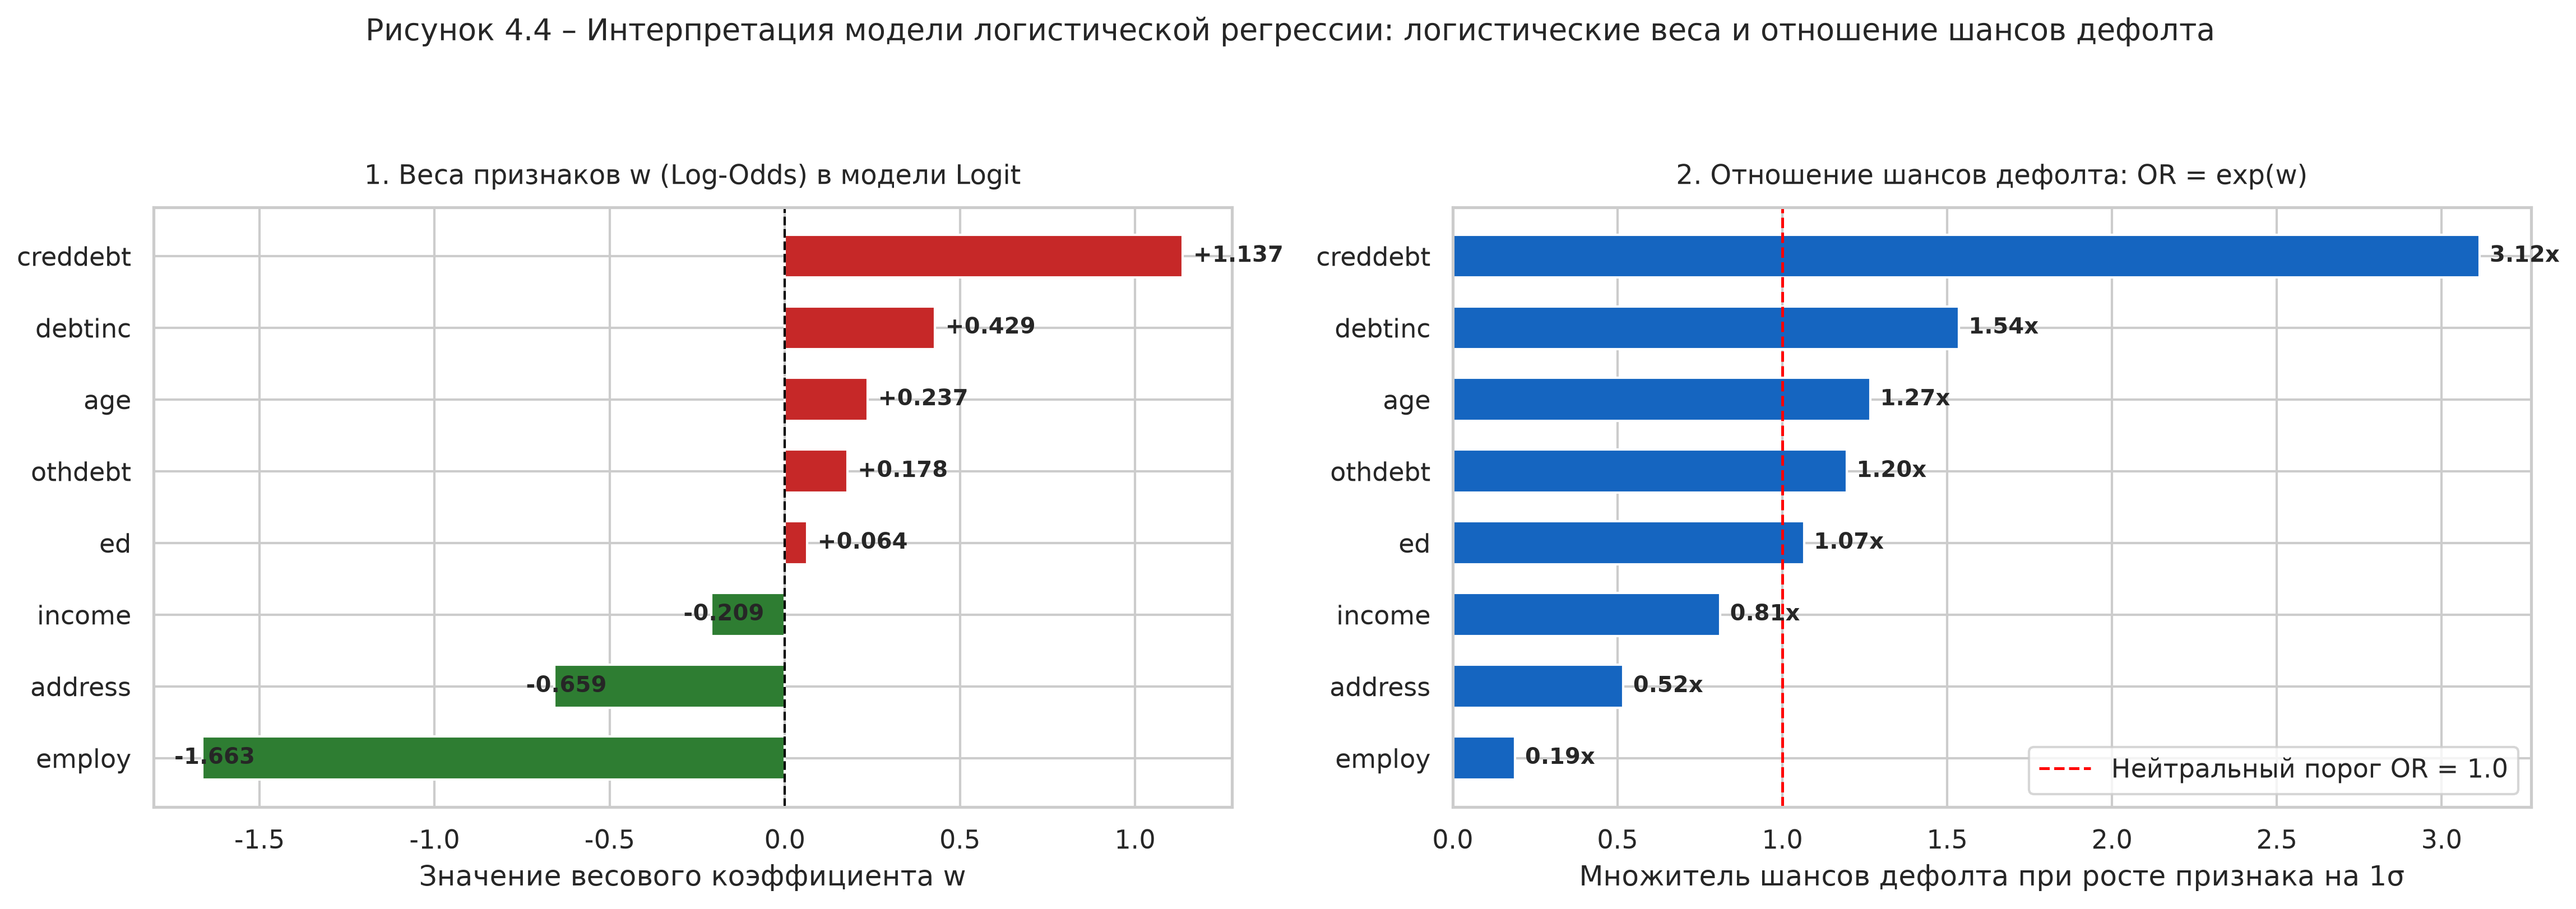
\includegraphics[width=0.92\textwidth]{plots/04_logistic_regression_analysis.png}
  \caption{Анализ коэффициентов логистической регрессии и распределение скоров}
\end{figure}

\subsection*{3. Метод опорных векторов (SVM: линейное и RBF ядра)}

На рисунке 5 сопоставлены решающие поверхности линейного и нелинейного гауссова (RBF) классификаторов SVM в проекции двух ключевых признаков (\texttt{debtinc} и \texttt{employ}). Линейный классификатор формирует широкий разделяющий зазор, эффективно отсекая зону риска, в то время как RBF-ядро строит замкнутые нелинейные изолинии вокруг кластеров дефолтных заемщиков.

\begin{figure}[H]
  \centering
  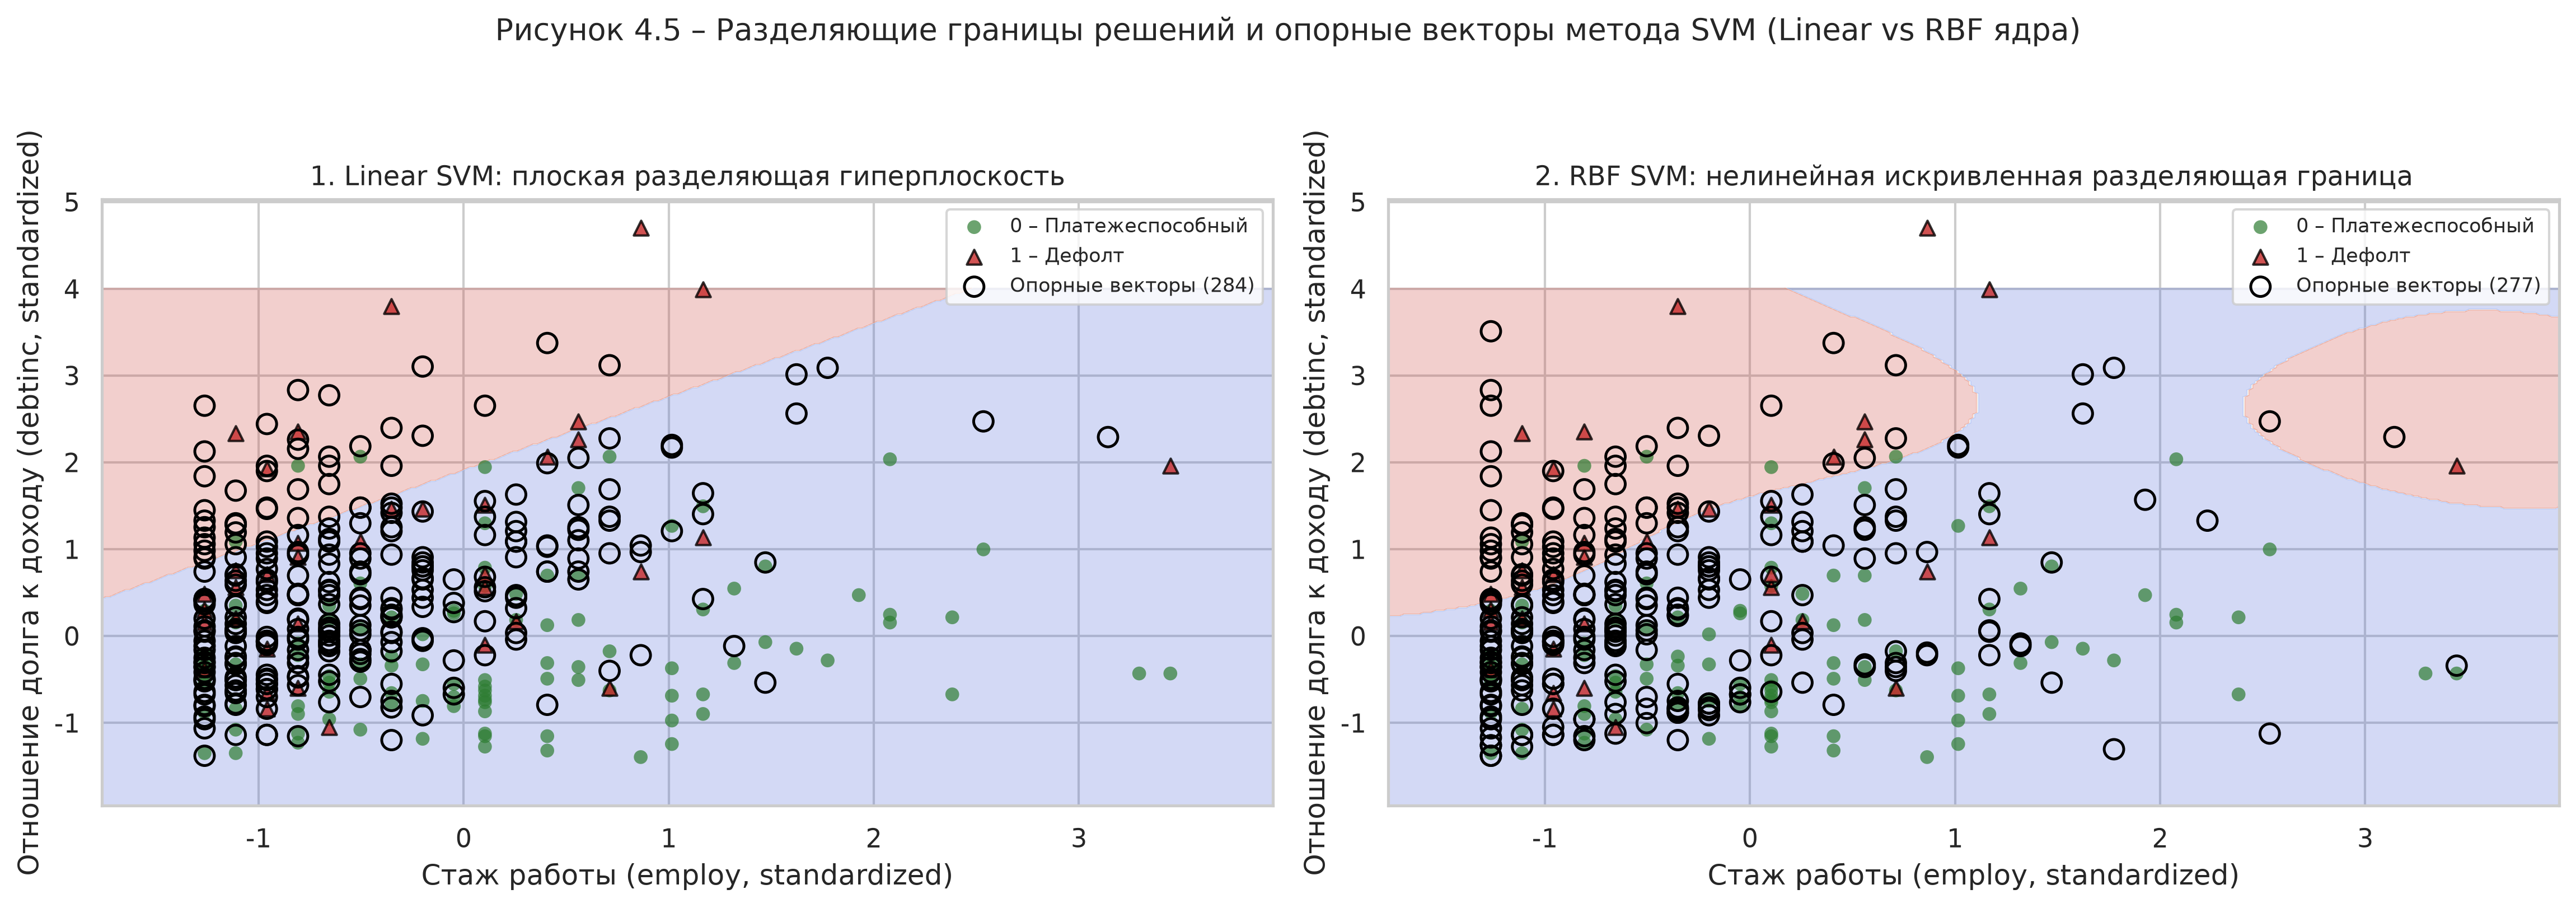
\includegraphics[width=0.92\textwidth]{plots/05_svm_decision_boundary_and_margins.png}
  \caption{Решающие поверхности и опорные векторы для Linear SVM и RBF SVM}
\end{figure}

\subsection*{4. Решающие деревья (CART)}

Для устранения риска переобучения глубина дерева CART была ограничена параметром \texttt{max\_depth=3}, а минимальный размер листа задан \texttt{min\_samples\_leaf=15}. Графическая структура построенного дерева приведена на рисунке 6. В качестве корневого признака алгоритм выбрал долговую нагрузку \texttt{debtinc} с порогом $14.7\%$, разделив клиентов на низкорисковую и высокорисковую когорты.

\begin{figure}[H]
  \centering
  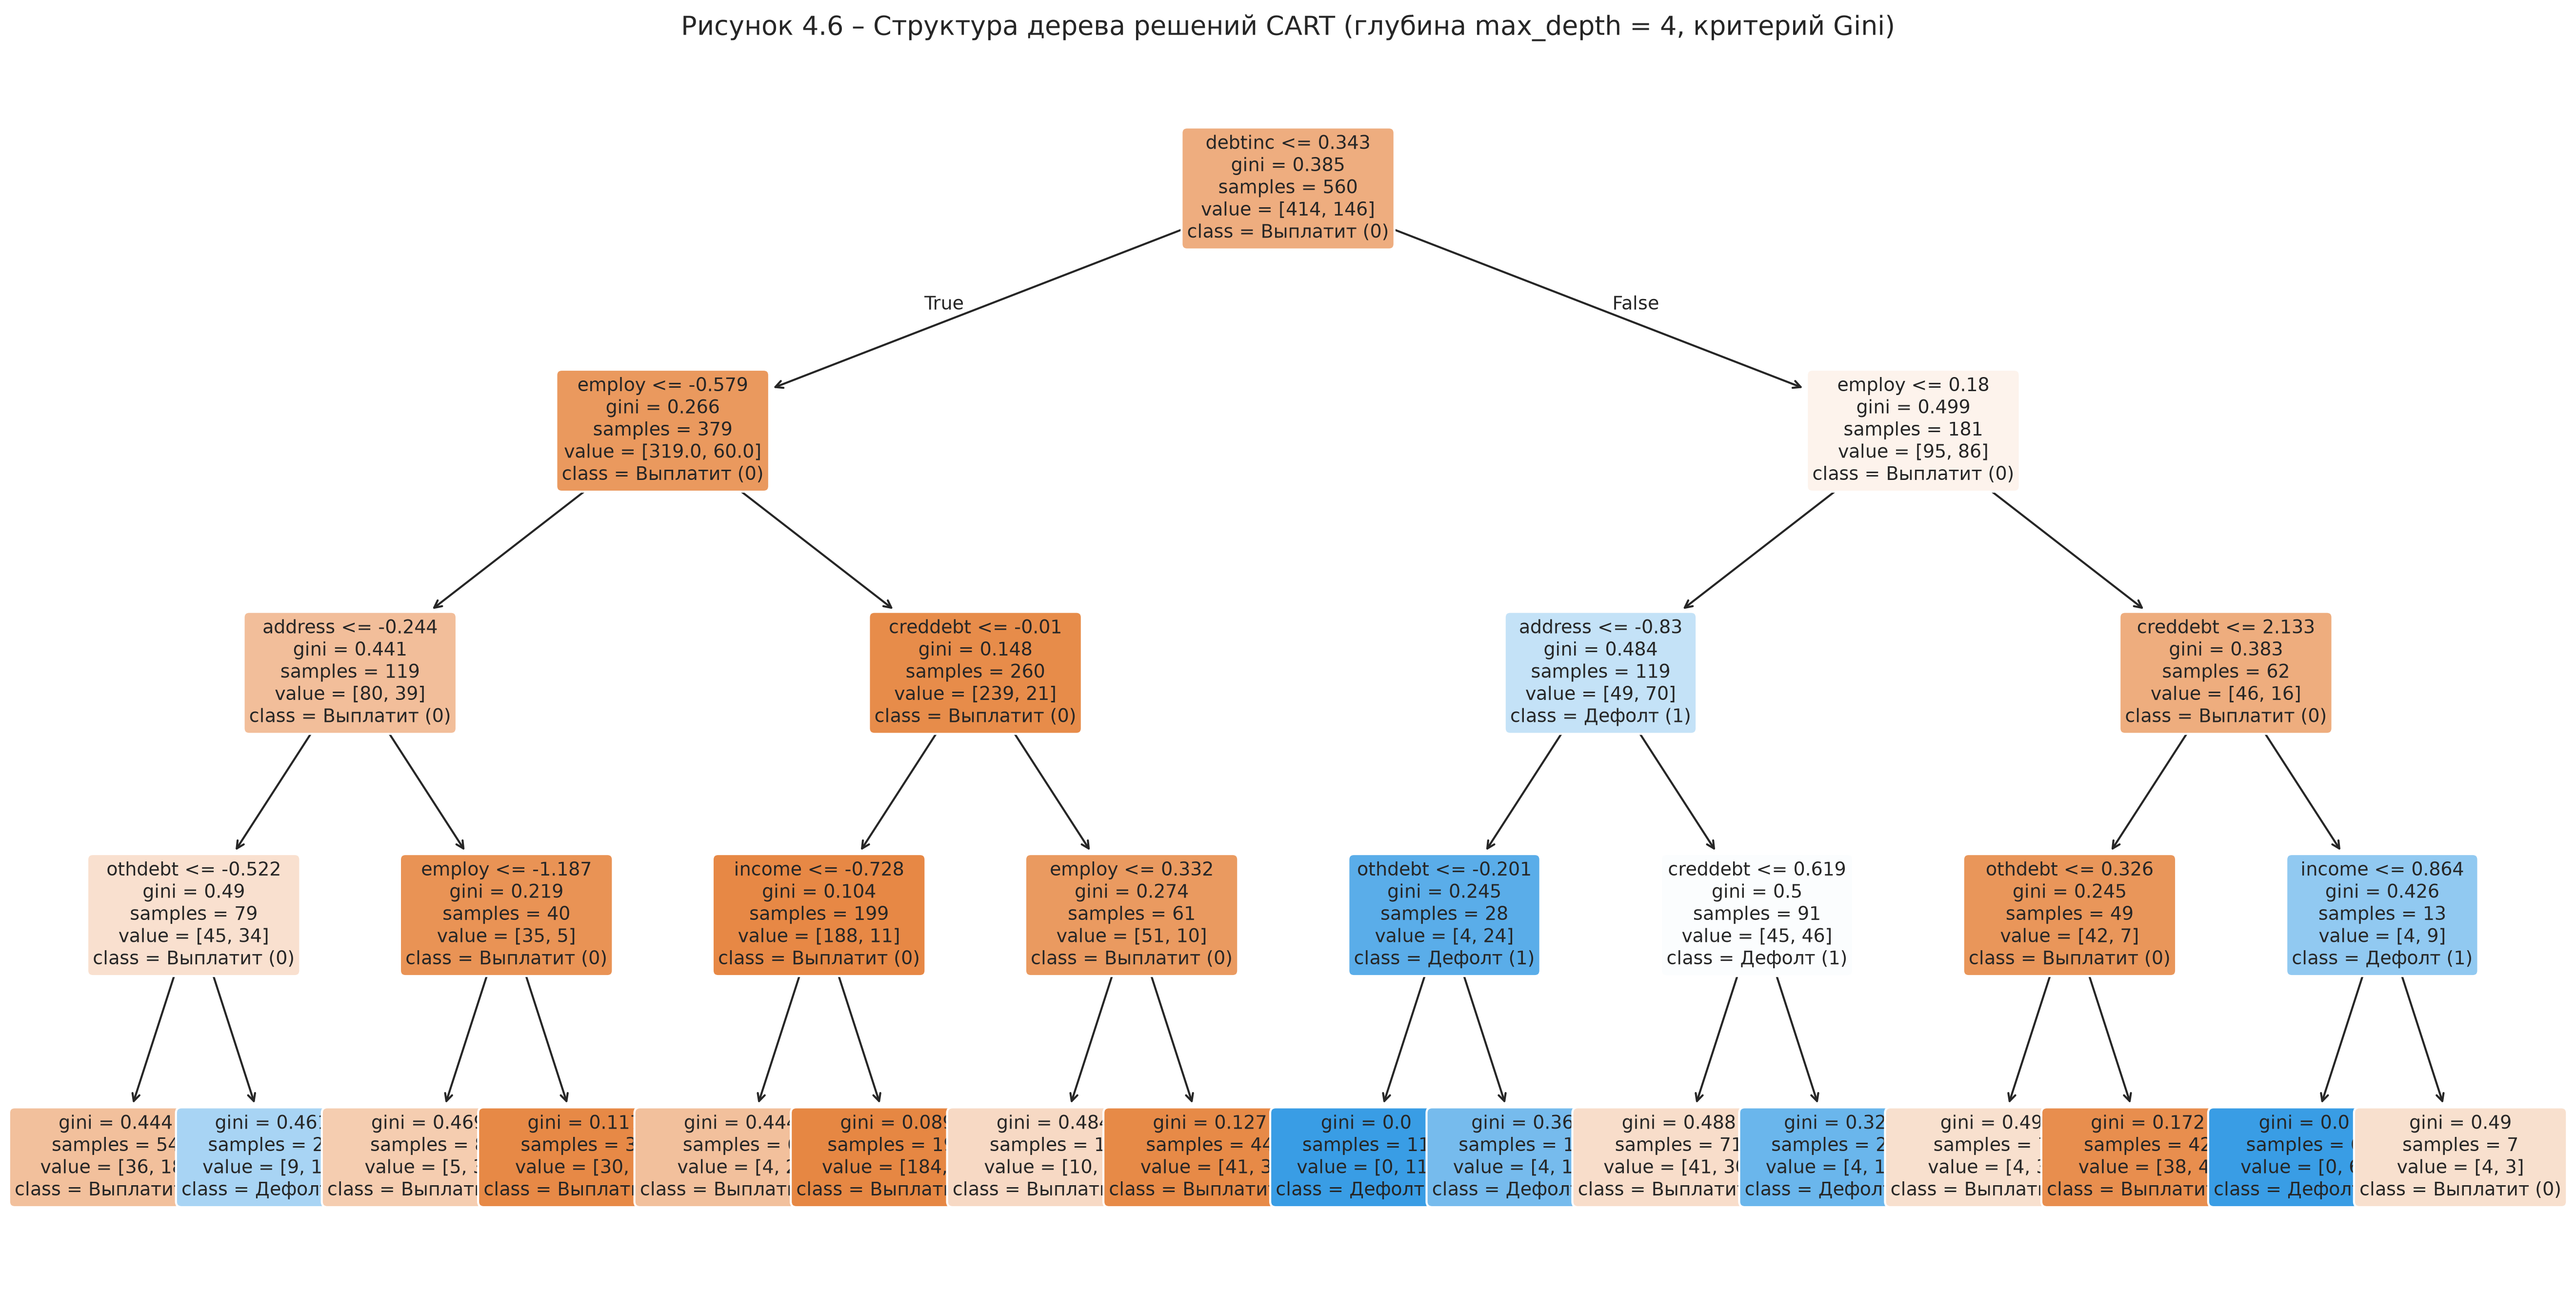
\includegraphics[width=0.94\textwidth]{plots/06_cart_decision_tree_visualization.png}
  \caption{Структура дерева решений CART с критерием Джини}
\end{figure}

\subsection*{5. Сравнительный анализ моделей}

На рисунках 7, 8 и 9 приведен комплексный сопоставительный анализ точности всех четырех обученных алгоритмов на независимой тестовой выборке ($n=140$).

\begin{figure}[H]
  \centering
  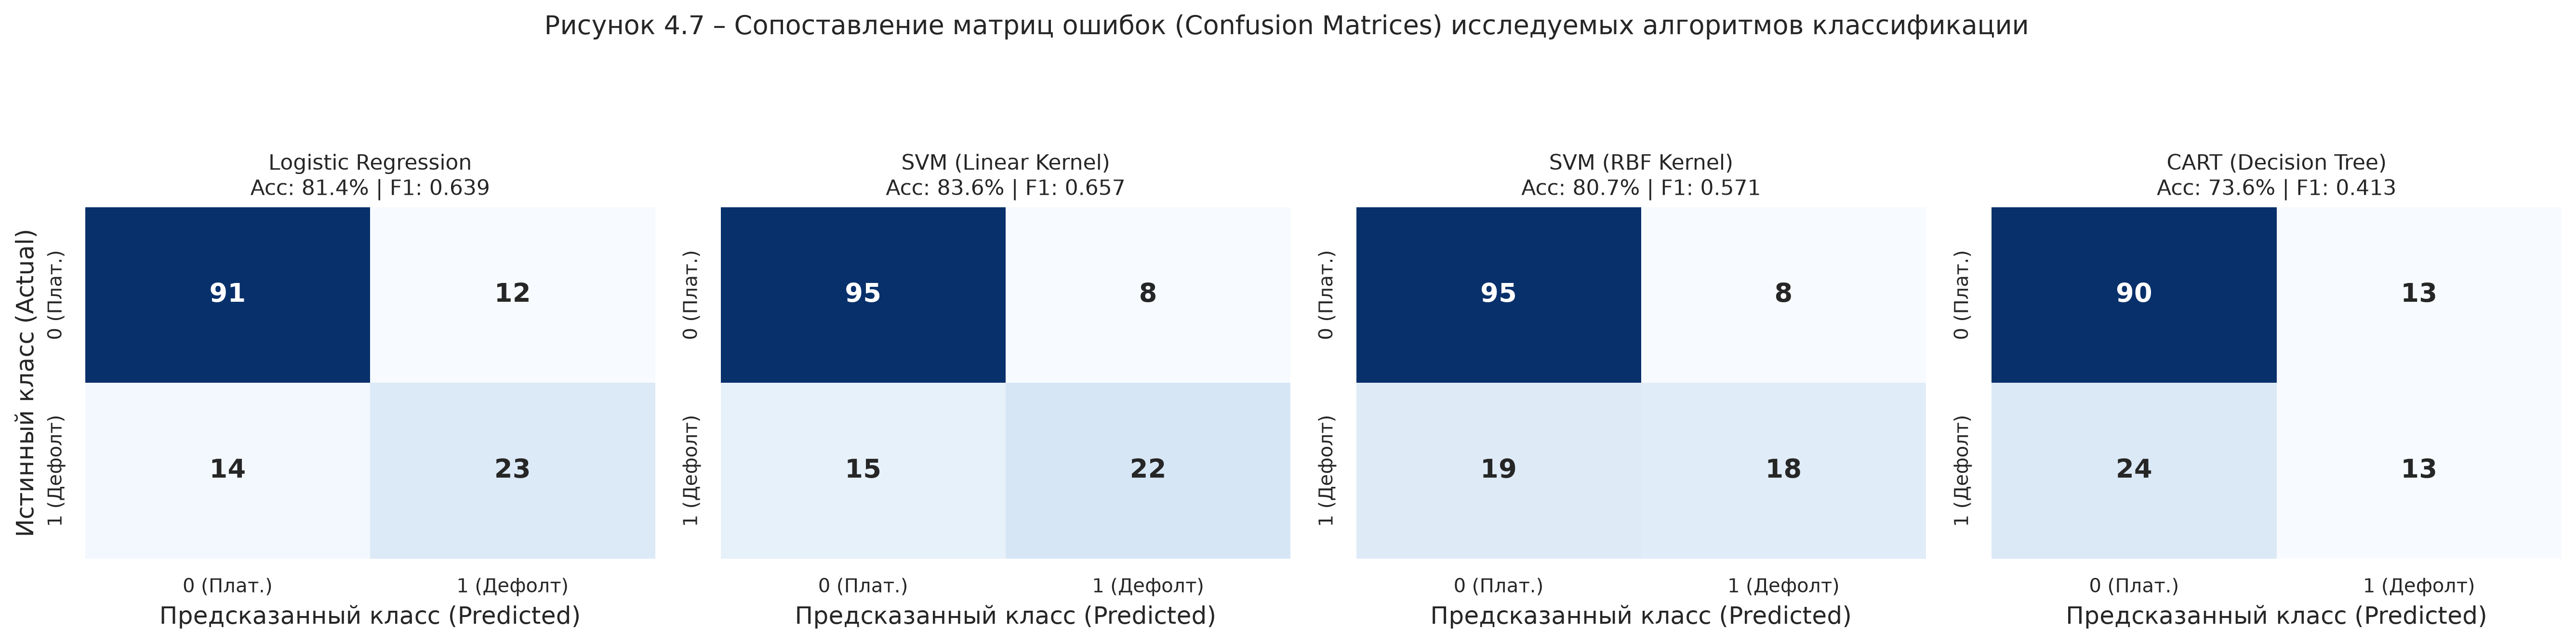
\includegraphics[width=0.92\textwidth]{plots/07_confusion_matrices_comparison.png}
  \caption{Матрицы ошибок (Confusion Matrices) на тестовой выборке}
\end{figure}

\begin{figure}[H]
  \centering
  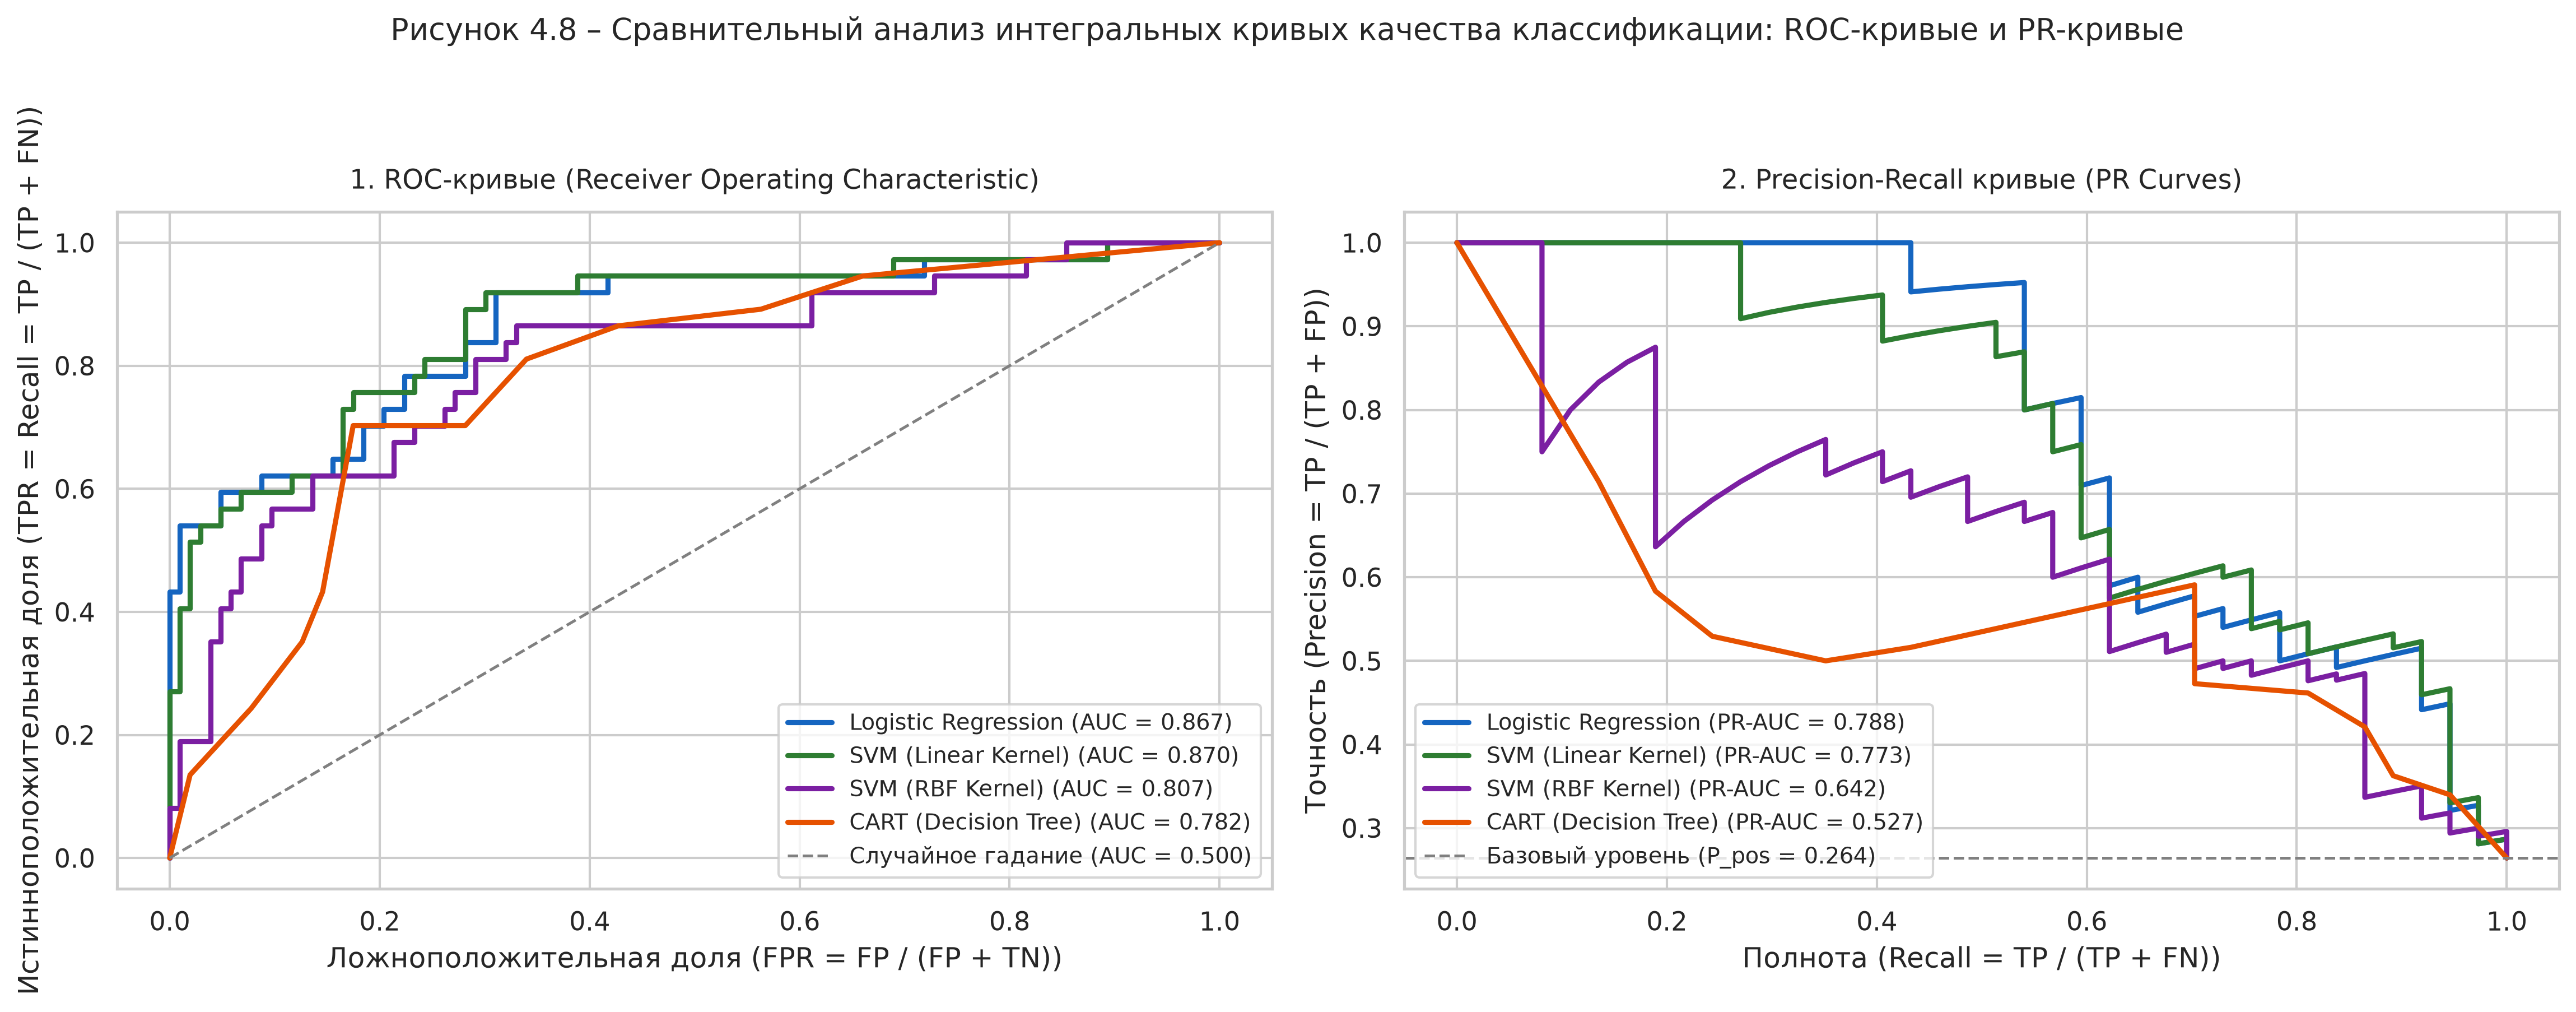
\includegraphics[width=0.92\textwidth]{plots/08_roc_and_pr_curves_comparison.png}
  \caption{ROC-кривые и кривые точности-полноты (Precision-Recall)}
\end{figure}

\begin{figure}[H]
  \centering
  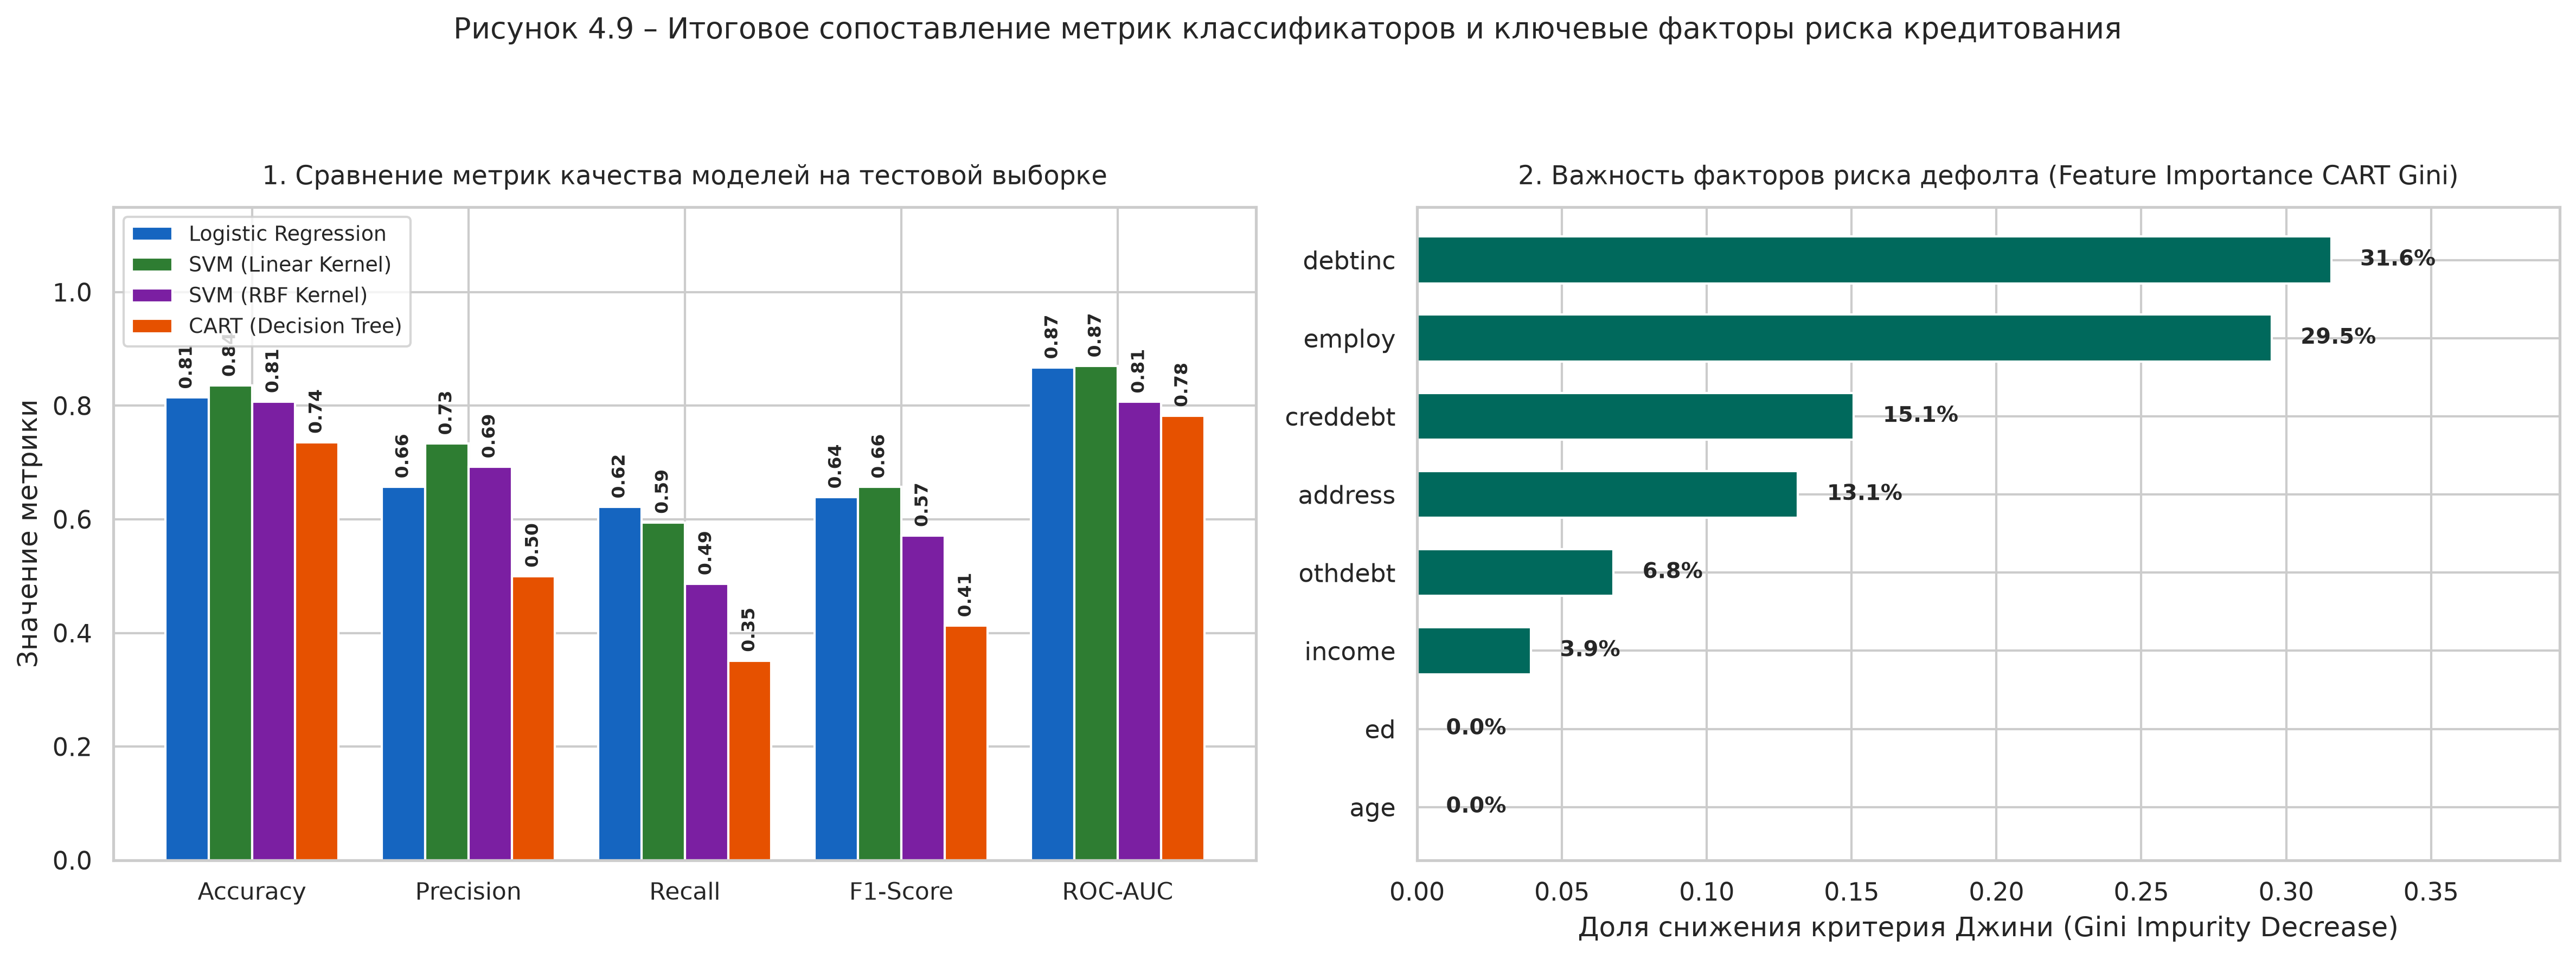
\includegraphics[width=0.92\textwidth]{plots/09_model_metrics_and_feature_importances.png}
  \caption{Сопоставление метрик качества и важности признаков}
\end{figure}

В таблице 1 сгруппированы итоговые численные показатели моделей.

\begin{table}[H]
\caption{Сравнительные метрики качества классификаторов на контрольной выборке}
\centering
\small
\begin{tabularx}{\textwidth}{lccccc}
\toprule
\textbf{Алгоритм} & \textbf{Accuracy} & \textbf{Precision} & \textbf{Recall} & \textbf{F1-score} & \textbf{ROC-AUC} \\
\midrule
Логистическая регрессия & 0.8143 & 0.6571 & \textbf{0.6216} & 0.6389 & 0.8670 \\
Linear SVM & \textbf{0.8357} & \textbf{0.7333} & 0.5946 & \textbf{0.6567} & \textbf{0.8699} \\
RBF SVM & 0.8071 & 0.6923 & 0.4865 & 0.5714 & 0.8066 \\
CART Decision Tree & 0.7357 & 0.5000 & 0.3514 & 0.4127 & 0.7825 \\
\bottomrule
\end{tabularx}
\end{table}

Наивысшую общую точность (Accuracy $83.57\%$), точность определения дефолта (Precision $73.33\%$) и показатель ROC-AUC ($0.8699$) продемонстрировал метод опорных векторов с линейным ядром (\texttt{Linear SVM}). При этом логистическая регрессия показала наивысшую полноту (Recall $62.16\%$), допустив наименьшее количество критических для банка ошибок второго рода (пропуск дефолтного клиента, $FN = 14$).

\subsection*{6. Скоринг кредитных заявок}

Применение откалиброванной модели логистической регрессии с консервативным порогом отсечения по вероятности дефолта $\tau = 0.35$ к пулу из 450 новых кандидатов позволило одобрить выдачу 336 кредитов ($74.7\%$) и отклонить 114 высокорисковых заявок ($25.3\%$).

% ==============================================================================
% ЛИСТИНГ КОДА
% ==============================================================================
\section*{ЛИСТИНГ ПРОГРАММНОГО КОДА}
\addcontentsline{toc}{section}{ЛИСТИНГ ПРОГРАММНОГО КОДА}

Ниже приведен ключевой фрагмент программной реализации на языке Python (библиотеки NumPy, Pandas, Scikit-Learn):

\begin{lstlisting}[language=Python]
import pandas as pd
import numpy as np
from sklearn.model_selection import train_test_split
from sklearn.preprocessing import StandardScaler
from sklearn.linear_model import LogisticRegression
from sklearn.svm import SVC
from sklearn.tree import DecisionTreeClassifier
from sklearn.metrics import classification_report, roc_auc_score

# 1. Загрузка и разделение выборки на обучающую и скоринговую
df = pd.read_csv('Bankloan.csv')
labeled_df = df[df['default'].notna()].copy()
unlabeled_df = df[df['default'].isna()].copy()

feature_cols = ['age', 'ed', 'employ', 'address', 'income', 'debtinc', 'creddebt', 'othdebt']
X = labeled_df[feature_cols]
y = labeled_df['default'].astype(int)

# 2. Стратифицированное разбиение и стандартизация
X_train, X_test, y_train, y_test = train_test_split(
    X, y, test_size=0.2, random_state=42, stratify=y
)
scaler = StandardScaler()
X_train_s = scaler.fit_transform(X_train)
X_test_s = scaler.transform(X_test)

# 3. Обучение классификаторов
lr = LogisticRegression(penalty='l2', C=1.0, random_state=42)
lr.fit(X_train_s, y_train)

svm_lin = SVC(kernel='linear', C=1.0, probability=True, random_state=42)
svm_lin.fit(X_train_s, y_train)

svm_rbf = SVC(kernel='rbf', C=1.0, gamma='scale', probability=True, random_state=42)
svm_rbf.fit(X_train_s, y_train)

cart = DecisionTreeClassifier(criterion='gini', max_depth=3, min_samples_leaf=15, random_state=42)
cart.fit(X_train, y_train)

# 4. Скоринг пула новых заемщиков
X_unlabeled_s = scaler.transform(unlabeled_df[feature_cols])
unlabeled_probs = lr.predict_proba(X_unlabeled_s)[:, 1]
unlabeled_preds = (unlabeled_probs >= 0.35).astype(int)
\end{lstlisting}

% ==============================================================================
% ЗАКЛЮЧЕНИЕ
% ==============================================================================
\section*{ЗАКЛЮЧЕНИЕ}
\addcontentsline{toc}{section}{ЗАКЛЮЧЕНИЕ}

В ходе выполнения лабораторной работы были всесторонне изучены и экспериментально исследованы базовые алгоритмы бинарной классификации данных в задаче оценки кредитоспособности заемщиков:
\begin{enumerate}
  \item Проведен разведочный анализ данных: подтверждено отсутствие скрытых пропусков, зафиксирован умеренный дисбаланс целевых классов ($26.1\%$ дефолтов), выявлены ключевые детерминанты неплатежеспособности --- соотношение долга к доходу (\texttt{debtinc}, $r = +0.39$) и стаж трудовой деятельности (\texttt{employ}, $r = -0.28$).
  \item Показано, что в стандартизированном пространстве признаков разделяющая поверхность между классами близка к квазилинейной. По этой причине линейный метод опорных векторов (\texttt{Linear SVM}) продемонстрировал наивысшую интегральную эффективность ($\text{ROC-AUC} = 0.8699, \text{Accuracy} = 83.57\%$), незначительно опередив логистическую регрессию ($\text{ROC-AUC} = 0.8670$).
  \item Модель логистической регрессии обеспечила наивысшую полноту охвата дефолтных событий ($\text{Recall} = 62.16\%$), а ее коэффициенты обладают строгой экономической интерпретацией в виде отношений шансов ($\text{Odds Ratios}$).
  \item Нелинейные модели (\texttt{SVM RBF} и решающее дерево \texttt{CART}) показали более скромные результаты на контрольной выборке ($\text{ROC-AUC} = 0.8066$ и $0.7825$ соответственно) вследствие высокой дисперсии и чувствительности к шуму на сравнительно небольшом наборе данных. При этом дерево CART предоставило прозрачную иерархию пороговых бизнес-правил с корневым ветвлением по порогу долговой нагрузки $14.7\%$.
  \item Успешно выполнен скоринг портфеля из 450 новых кредитных заявок с консервативной риск-политикой, обеспечивающей минимальный уровень потенциальных невозвратов кредитных средств.
\end{enumerate}

% ==============================================================================
% СПИСОК ИСПОЛЬЗОВАННЫХ ИСТОЧНИКОВ
% ==============================================================================
\section*{СПИСОК ИСПОЛЬЗОВАННЫХ ИСТОЧНИКОВ}
\addcontentsline{toc}{section}{СПИСОК ИСПОЛЬЗОВАННЫХ ИСТОЧНИКОВ}

\begin{enumerate}
  \item Вьюгин, В. В. Математические основы машинного обучения и прогнозирования / В. В. Вьюгин. --- М.: МЦНМО, 2013. --- 390 с.
  \item Hastie, T. The Elements of Statistical Learning: Data Mining, Inference, and Prediction / T. Hastie, R. Tibshirani, J. Friedman. --- 2nd ed. --- New York: Springer, 2009. --- 745 p.
  \item Bishop, C. M. Pattern Recognition and Machine Learning / C. M. Bishop. --- New York: Springer, 2006. --- 738 p.
  \item Рашка, С. Python и машинное обучение / С. Рашка, В. Мирджалили. --- СПб.: Диалектика, 2020. --- 848 с.
  \item Scikit-learn: Machine Learning in Python / F. Pedregosa [et al.] // Journal of Machine Learning Research. --- 2011. --- Vol. 12. --- P. 2825--2830.
\end{enumerate}

\end{document}
